\section {Software Products} \label{sec:softproducts}
The DM products are not data as many may think, rather the products are software and services to produce those
products.
In operations DM will not exist though an analogous organization called Data Production will spring into existence under similar leadership.


The high level list of DM products is given in \figref{fig:pt}, as may be seen in the  figure we consider software, services and systems (enclaves) as products.


\begin{figure}
\begin{centering}
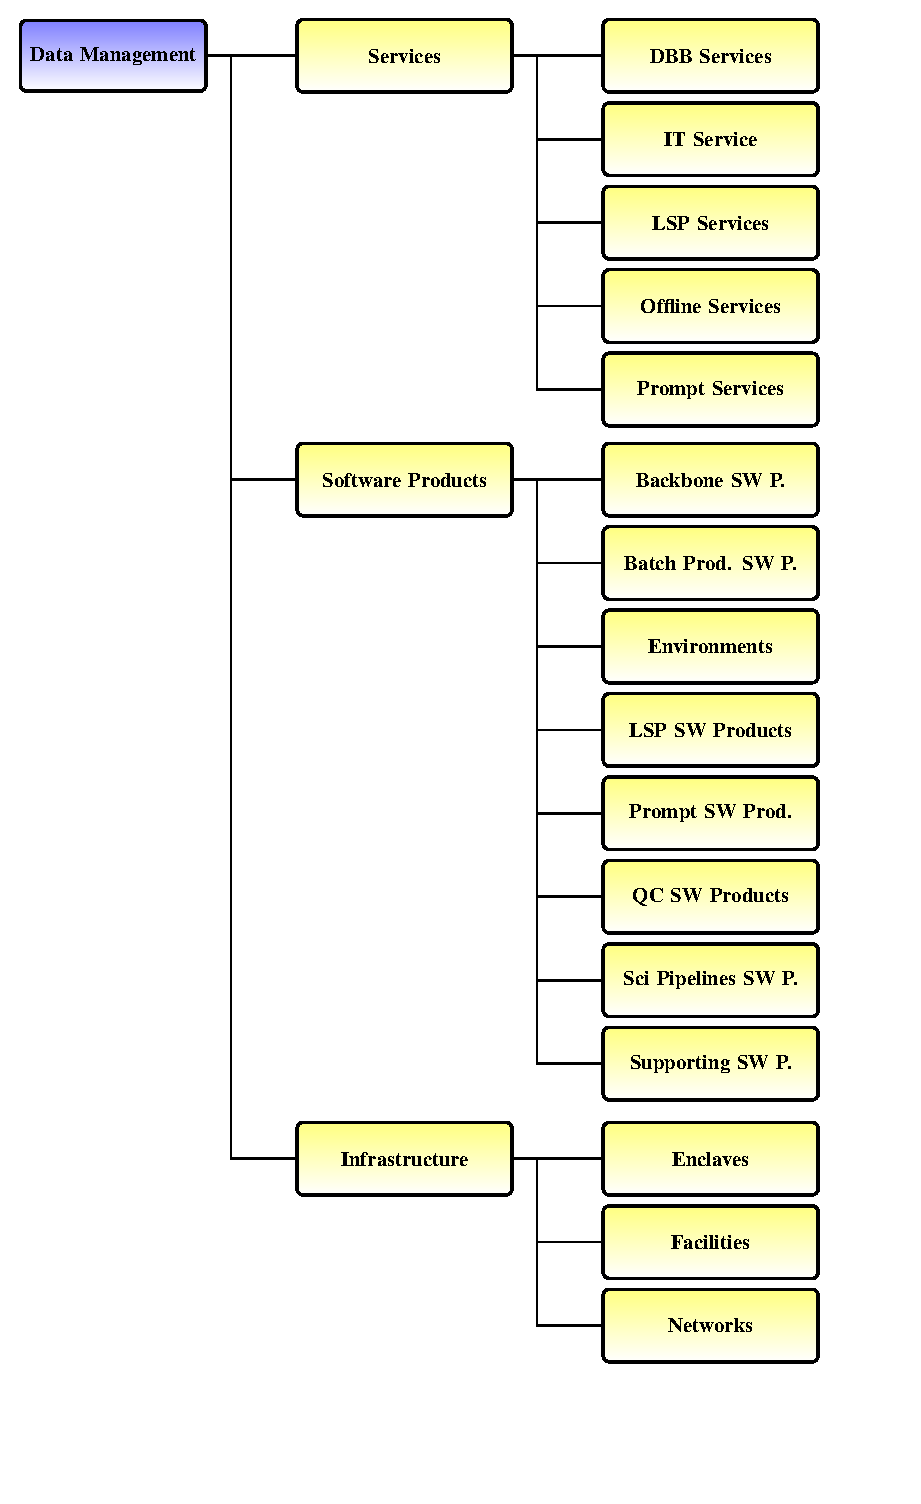
\includegraphics[width=0.9\textwidth]{images/ProductTree}
	\caption{Rubin DM product tree \label{fig:pt}}
\end{centering}
\end{figure}



\subsection{Commissioning Software Products}
A detailed section describing what we delivered and used to process the commissioning data.
This section will probably not be written until  commissioning.

\subsection{Anticipated Data Release 1 Software Products}
A short section describing what we anticipate delivering  for DR1 in addition to what was delivered in commissioning.
This section will probably not be written until after commissioning.

\subsection{Science Pipelines}\label{sec:pipes}
The science pipelines which produce the prompt and data release products are of course the most identifiable
software product from DM.
The detailed approach to Science Pipelines is covered in \cite{PSTN-019}.


\subsection{Science Platform}

\subsection{Services}
